\title{Answers to Problem Set 1}
\author{
				Lauren Hinkle (lhinkle)\\
        Pedro d'Aquino  (pdaquino)\\
				Robert Goeddel (rgoeddel)\\
        Yash Chitalia (yashc)}
\date{\today}

\documentclass[12pt]{article}
\usepackage{graphicx}
\usepackage{amsmath}

\begin{document}
\maketitle

\section{Task 1: Linear Algebra Review}

\paragraph{A}
Let $A$ be a matrix with the property $AA^T = I$ where $A$ is an $m\times n$ matrix.  Then it must be that $r_i$ is orthogonal to $r_j$ for all rows $r_i, r_j \in A$.  Additionally, $m \leq n$, this is explained in 1C.

\paragraph{B}
\begin{equation*}
A = \left[ \begin{array}{ccc} 1 & 0 & 0 \\ 0 & 1 & 0 \end{array} \right]
\end{equation*}

Proof: \\
\begin{align*}
AA^T:\hspace{10 mm}
\left[ \begin{array}{ccc} 1 & 0 & 0 \\ 0 & 1 & 0 \end{array} \right]
\left[ \begin{array}{cc} 1 & 0  \\ 0 & 1 \\ 0 & 0 \end{array} \right]
&=\left[ \begin{array}{cc} 1 & 0  \\ 0 & 1 \end{array} \right] \\
A^TA:\hspace{10 mm}
\left[ \begin{array}{cc} 1 & 0  \\ 0 & 1 \\ 0 & 0 \end{array} \right]
\left[ \begin{array}{ccc} 1 & 0 & 0 \\ 0 & 1 & 0 \end{array} \right]
&=\left[ \begin{array}{ccc} 1 & 0 & 0  \\ 0 & 1 & 0 \\ 0 & 0 & 0 \end{array} \right]
\end{align*}


\paragraph{C}
Let $A$ be an $m \times n$ matrix such that $AA^T=I$. We can decompose $AA^T$ using SVD:

\[
AA^T = USV^T\left(USV^T\right)^T = USV^TVS^TU^T\]

Because $V$ is orthonormal, $VV^T=I$ and:

\[
AA^T = USS^TU^T
\]

For $AA^T=I$, $SS^T=I$. This follows from the fact that $U$ is orthonormal.

If we expand $A^TA$ using SVD, we reach:

\[
A^TA = VS^TSV^T
\]

For $A^TA$ to be $I$, then $S^TS=I$. But we know that $SS^T$ is also $I$, so these conditions must hold simultaneously for $A^TA=I$.

Recall that $S$ is diagonal and has the same dimensions as $A$. If it is also square, then those conditions can hold simultaneously because $SS^T=S^TS$. However, if $S$ is rectangular, at least one row or column will have nothing but zeroes. In this case, there is only one direction in which multiplying $S$ and $S^T$ yields $I$; in the other direction the result will be a square matrix with at least one row and column equal to zero.

\paragraph{D}
Classes of matrices for which $AA^T = I$ and $A^TA=I$ will hold are square matrices, orthogonal (by definition of an orthogonal matrix), and symmetric.

\section{Task 2: Multiavariate Gaussians}

\paragraph{A}
Let $N$ be the number of samples, $K$ be the number of random variables in $\mathbf{x}$ and $\mathbf{\mu}$ be the sample mean vector. The $i$-th sample of the random variable $\mathbf{x}_k$ is denoted by $\mathbf{x}_{ik}$ Then each element of $\mathbf{\mu}$ is going to be of the form:

\begin{equation}
\mu_k = \frac{1}{N}\displaystyle\sum_{i=1}^{N}{x_{ik}}, k=1,2,...,K
\end{equation}

And every element $\sigma_{jk}$ of the $K \times K$ covariance matrix $\Sigma$ will be given by:

\begin{equation}
\sigma_{jk}=\frac{1}{N-1}\displaystyle\sum_{i=1}^{N}{(x_{ij}-\mu_j)(x_{ik}-\mu_{k})}
\end{equation}

\paragraph{B}

We first prove that for any $m \times n$ matrix $A$, $AA^T$ is SPD. Let $x$ be any column vector of dimensions $m\times1$ and let

\[
\underbrace{x^T}_{1\times m}\underbrace{A}_{m\times n}=\underbrace{t}_{1\times n}
\]

Then:

\[
x^TAA^Tx = \underbrace{t}_{1\times n}\underbrace{t^T}_{n \times 1} = \underbrace{s}_{1\times 1}
\]

Additionaly, $s\geq 0$:

\[s = \displaystyle\sum_{i=1}^n{t_i^2}\]

Therefore, $AA^T$ is SPD. We can extend this to prove that any covariance matrix is also SPD. Again, let$x$ be any column vector of dimensions $m\times1$. We need to prove that $x^T\Sigma x \geq 0$.

\[
x^T\Sigma x=x^TE\left[\left(X-E[X]\right)\left(X-E[X]\right)^T\right]x
\]

Let $A=X-E[X]$. Then we rewrite the equation as:

\[
x^T\Sigma x=x^TE\left[AA^T\right]x = E\left[x^TAA^Tx\right]
\]

But we have already proved that $x^TAA^Tx$ is a scalar $s$, $s \geq 0$:

\[
x^T\Sigma x  =E\left[s\right] \geq 0
\]

\paragraph{C}
Let $Z$ be a multivariate distribution comprised of independent standard normal univariate distributions. Then the mean $\mu_Z = 0$ and the covariance $\Sigma_Z=I$, the identity matrix. If we apply a linear transformation of the form $AZ + b$, we will have a multivariate normal distribution of the form:

\[
\mathcal{N}\left(A\mu_Z + b, A\Sigma_Z A^T\right) = \mathcal{N}\left(A0 + b, BIB^T\right) = \mathcal{N}\left(b, AA^T\right)
\]

Therefore, we can draw from $\mathcal{N}\left(\mu,P\right)$ by making $b=\mu$ and $AA^T=P$ (using, for instance, Cholesky decomposition).

\paragraph{D}
Let there be a two-dimensional distribution with given covariance $\Sigma$ such that there is a $\chi^2$ error of $c$ for some point $p$ where $p = \mu +
\left[ {\begin{smallmatrix}
\alpha cos(\theta)  \\
\alpha sin(\theta)  \\
 \end{smallmatrix} } \right]$
with a given value of $\theta$ and unknown $\alpha$.

By definition, $\chi^2 = \mathbf{w}^T \Sigma^{-1} \mathbf{w}$ where $\mathbf{w} = \mathbf{p}-\mathbf{\mu}$.  Then
\begin{align*}
\mathbf{w} &= \mu +
	\left[ {\begin{smallmatrix}
	\alpha cos(\theta)  \\
	\alpha sin(\theta)  \\
 	\end{smallmatrix} } \right]
	- \mu \\
 &= \alpha \left[ {\begin{smallmatrix}
	cos(\theta)  \\
	sin(\theta)  \\
	 \end{smallmatrix} } \right]
\end{align*}
And therefore the unknown $\alpha$ can be calculated.
\begin{align*}
\chi^2 = c &=  \mathbf{w}^T \Sigma^{-1} \mathbf{w} \\
&=  \alpha \left[ {\begin{smallmatrix}
	cos(\theta)  sin(\theta)  \\
	 \end{smallmatrix} } \right]
 	\Sigma
 	\alpha \left[ {\begin{smallmatrix}
	cos(\theta)  \\
	sin(\theta)  \\
	 \end{smallmatrix} } \right] \\
&= \alpha^2 \left[ {\begin{smallmatrix}
	cos(\theta)  sin(\theta)  \\
	 \end{smallmatrix} } \right]
 	\Sigma
 	\left[ {\begin{smallmatrix}
	cos(\theta)  \\
	sin(\theta)  \\
	 \end{smallmatrix} } \right] \\
\alpha^2 &= \frac{c}{\left[ {\begin{smallmatrix}
	cos(\theta)  sin(\theta)  \\
	 \end{smallmatrix} } \right]
 	\Sigma
 	\left[ {\begin{smallmatrix}
	cos(\theta)  \\
	sin(\theta)  \\
	 \end{smallmatrix} } \right]} \\
\alpha &=\pm\sqrt{ c \left( \left[ {\begin{smallmatrix}
	cos(\theta)  sin(\theta)  \\
	 \end{smallmatrix} } \right]
 	\Sigma
 	\left[ {\begin{smallmatrix}
	cos(\theta)  \\
	sin(\theta)  \\
	 \end{smallmatrix} } \right]
	 \right)^{-1}}
\end{align*}


\paragraph{E}
NOTE: Run team.MultiGaussian to see our tests live.

To test that our sample mean/covariance code generated sane results,
we calculated an example by hand and then compared to the actual results.
In this case, we did the small case of the points:

\[(0,1) (1,0) (1,1)\]

By our prediction, the sample mean should come out to be $(\frac{2/3}, \frac{2/3})$
and the sample covariance

\begin{figure}
\centering
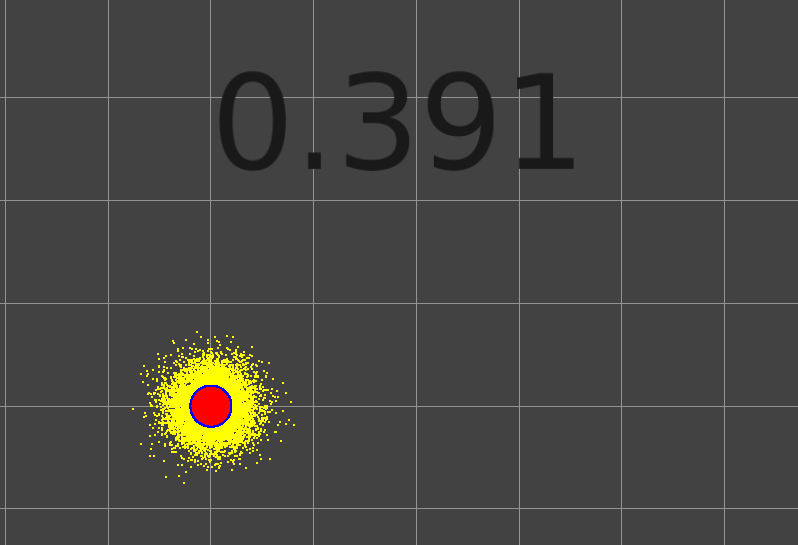
\includegraphics[width=0.8\textwidth]{figures/MultiGaussian_1_sigma.png}
\label{fig:multigaussian}
\caption{Around 39\% of our sampled points fell within our ellipse for $\chi^{2} = 1$.}
\end{figure}

\section{Task 3: Covariance Matrices and Covariance Projection}

\paragraph{A}

We first write $x$ and $y$ in terms of $r$ and $\theta$:

\[x = r\cos\theta\]
\[y = r\sin\theta\]


The covariance matrix in terms of $x$ and $y$ can be expressed in terms of the original covariance matrix as follows:

\[
\Sigma_{x,y} = J_{r,\theta}^{x,y}|_{r_0,\theta_0} \Sigma_{r,\theta}\left(J_{r,\theta}^{x,y}|_{r_0,\theta_0}\right)^T
\]

Where:

\[
J_{r,\theta}^{x,y} =
\left[ {\begin{array}{cc}
	\frac{\partial r}{\partial x}|_{r_0} & \frac{\partial \theta}{\partial x}|_{\theta_0}  \\[5pt]
	\frac{\partial r}{\partial x}|_{r_0} & \frac{\partial \theta}{\partial x}|_{\theta_0}  \\[5pt]
	 \end{array} } \right] =
\left[ {\begin{array}{cc}
	\cos\theta_0 & -r\sin\theta_0  \\
	\sin\theta_0 & r\cos\theta_0  \\
	 \end{array} } \right]
\]
\[
\Sigma_{r,\theta} =
\left[ {\begin{array}{cc}
	50 & 0  \\
	0 & 15 \end{array} }\right]
\]

Therefore,

\[
\Sigma_{x,y} = \left[ {\begin{array}{cc}
	\cos\theta_0 & -r_0\sin\theta_0  \\
	\sin\theta_0 & r_0\cos\theta_0  \\
	 \end{array} } \right]
	 	\left[ {\begin{array}{cc}
	50 & 0  \\
	0 & 15 \end{array} }\right]
	\left[ {\begin{array}{cc}
	\cos\theta_0 & \sin\theta_0  \\
	-r_0\sin\theta_0 & r_0\cos\theta_0  \\
	 \end{array} } \right] \]
\[
\Sigma_{x,y} = \left[ {\begin{array}{cc}
		50\cos^2\theta_0 + 0.15r_0^2\sin^2\theta_0 & 50\cos\theta_0\sin\theta_0 - 0.15r_0^2\cos\theta_0\sin\theta_0  \\[5pt]
	50\cos\theta_0\sin\theta_0 - 0.15r_0^2\cos\theta_0\sin\theta_0 & 50\sin^2\theta_0 + 0.15r_0^2\cos^2\theta_0 \\[5pt]
	 \end{array} } \right] 
\]

\paragraph{B}


\end{document}
